\createTitlePage{فصل سوم}{تولید جمله}
\subsection{تولید جمله}
در این بخش، به بررسی چالش تولید جمله و روش‌های پیشنهاد شده برای حل این چالش، در طول زمان، خواهیم پرداخت. در ابتدا ایده‌های اولیه در این مسیر را بیان نموده و به طور خلاصه مورد بحث قرار خواهیم داد و در ادامه به بررسی تفصیلی روش‌های مبتنی بر استفاده از شبکه‌های عصبی بازگشتی در تولید جملات زبان طبیعی، می‌پردازیم.
\\
 چالش تولید جمله، متوجه ساخت جملاتی به زبان طبیعی است، به طوری‌که از لحاظ دستور زبان، املا و معنا صحیح باشند. از طرفی با توجه به هدف اصلی ما که تولید شرح بر تصاویر است، جملات تولید شده باید علاوه بر این‌که شرط صحت مذکور را ارضا می‌کنند، با تصویر ورودی، صحنه توصیف شده در تصویر و رخ‌داد به نمایش کشیده شده، هم‌خوانی داشته باشند. تضمین این هم‌خوانی از جمله معضلات دیگری است که باید برای آن چاره‌ای اندیشید.
\\
مساله تولید خودکار جملات زبان طبیعی، یکی از مسائلی است که از دیرباز در هوش مصنوعی مطرح بوده و دارای کاربردهای فراوانی است. به عنوان یک تعریف دقیق از این مساله، می‌توان به «فرایند تولید جملات زبان طبیعی با استفاده از داده‌های غیر قابل تفسیر برای کاربران عادی در جهت افزایش قابلیت تفهیم داده‌ به آن‌ها \cite{reiter1997building}» اشاره کرد. داده‌های اولیه که جملات با استفاده از آن‌ها تولید می‌شوند، می‌توانند شامل انواع داده‌های غیر متنی از جمله نمودارها، تصاویر، اعداد و مواردی از این دست باشند.
\\
در ادامه، ابتدا کاربردهای مساله تولید خودکار جملات زبان طبیعی\enfootnote{Natural Language Generation (NLG)}، خواهیم پرداخت.


\subsection[کاربردها\cite{reiter1997building}]{کاربردها}
کاربردهای بسیار زیاد و متنوعی برای تولید خودکار جملات زبان طبیعی با استفاده از داده‌های غیر متنی، ارائه شده است. در این بخش، برای روشن شدن اهمیت این مساله، تعدادی از این کاربردها را بیان خواهیم نمود.
\\
\begin{enumerate}
\item
تولید خودکار شرح بر پیش‌بینی وضع آب و هوا با استفاده از نقشه‌های گرافیکی آب و هوا
\item 
تولید خلاصه‌ای در باره داده‌های آماری استخراج شده از یک پایگاه داده 
\item
توصیف یک زنجیره استدلالی، منتج از فرایند تصمیم‌گیری یک سیستم خبره
\item
تولید پاسخ برای پرسش‌ها در مورد یک جسم در یک سامانه مبتنی بر دانش
\end{enumerate}

موارد ذکر شده در بالا، تنها نمونه‌ای از کاربردهای وسیع این مساله در زندگی‌های روزمره را نمایش می‌دهد.

%%%%%%%%%%%%%%%%%%%%%%%%%%%%%%%%%%%%%%%%%%%%%%%%%%%%%%%%%%%
%\subsection{روش‌های مختلف موجود}


%%%%%%%%%%%%%%%%%%%%%%%%%%%%%%%%%%%%%%%%%%%%%%%%%%%%%%%%%%
\subsection{روش‌ تولید زبان طبیعی}

یکی از حوزه‌های پویا در زمینه هوش مصنوعی و پردازش متن، حوزه تولید زبان طبیعی است. این حوزه شامل فعالیت‌هایی است که به تولید جمله زبان طبیعی متناظر با داده‌های قابل تفسیر برای ماشین مانند پایگاه‌های دانش 
\enfootnote{Knowledge Bases}
و یا قالب‌های منطقی\enfootnote{Logical Forms}
و مواردی از این دست، می‌‌پردازد. روش‌های کلی که در چارچوب کاری\enfootnote{Framework}  پژوهش‌های این زمینه مورد استفاده قرار می‌گیرد، به ‌طور کلی شامل مراحل زیر است\cite{reiter1997building}.

\begin{enumerate}
\item برنامه‌ریزی متن\enfootnote{Text Planning}
\\
در این مرحله، ابتدا محتوای مورد نیاز، انتخاب می‌‌شود و چارچوب کلی برای کل متن، طرح‌ریزی می‌شود. انتخاب محتوا و طرح‌ریزی چارچوب کلی متن، با تکیه بر کاربرد مورد نظر در پژوهش و داده‌هایی که نیاز به تفسیر زبانی دارند، انجام می‌شود.
\item برنامه‌ریزی جمله\enfootnote{Sentence Planning}
\\
در این مرحله، کلمات مورد نیاز انتخاب می‌شوند، عبارات زبانی مناسب تولید می‌شوند و به طور دقیق کنارهم قرار می‌گیرند تا جملات را تشکیل دهند. انتخاب کلمات و ساخت عبارات در این بخش، بر اساس طرح کلی پی‌ریزی شده برای متن در مرحله قبل، انجام می‌شود. کنارهم قرار دادن عبارات زبانی مورد نیاز نیز، با استفاده از قواعد دستور زبان که عموما به شکل پایگاه دانش موجود است، انجام می‌گردد.
\item تحقق زبانی\enfootnote{Linguistic Realisation}
\\
در این مرحله، که مرحله نهایی است، پردازش‌های شامل پردازش‌های نحوی\enfootnote{Syntactic} برای صیقل‌دادن جملات تولید شده و تصحیح نهایی آن‌ها،‌ صورت می‌گیرد.
\end{enumerate}


اولین روش‌های ارائه شده در این حوزه، عموما محدود به کاربردهای خاص بودند. در عموم این روش‌ها، مراحل مورد نیاز برای اجرای فرایند تولید جمله به ترتیب زیر، اجرا می‌شدند.
\\
\begin{enumerate}
\item استخراج لغات متناظر با داده از طریق جدول نگاشت ثابت\enfootnote{Hardcoded Mapping Table}
\item استخراج عبارات مناسب زبانی برای تولید جمله
\item اعمال قوانین دستور زبان برای ساخت جمله
\end{enumerate}

 در \cite{reiter1997building}، روشی برای تولید جملات زبان طبیعی، بیان‌کننده وضعیت حرکت قطارها در یک ترمینال مسافربری، ارائه داده است. در این پژوهش، اطلاعات مختلف موجود در پایگاه داده، به دو دسته پیام‌های «حرکت از مبدا» و «رسیدن به مقصد» تقسیم می‌شوند و اطلاعات زمانی و شماره هر قطار در هر پیام، استخراج می‌شود. سپس با استفاده از یک جدول از پیش تعیین شده ثابت\enfootnote{Hardcoded Mapping Table}، هر پیام به یک مجموعه از لغات، نگاشت می‌شود. در ادامه، عبارات زبانی مناسب جهت تولید جملات استخراج شده و با اعمال کلیشه‌های ثابت\enfootnote{Fixed Templates} ، جملات نهایی تولید می‌شوند.

 
%%%%%%%%%%%%%%%%%%%%%%%%%%%%%%%%%%%%%%%%%%%%%%%%%%%%%%%%%%
\subsection{روش نزدیک‌ترین همسایه}

یکی از پرکاربردترین روش‌ها در این زمینه، استفاده از روش نزدیک‌ترین همسایه است. در این روش، با استفاده از بردار ویژگی‌های به دست‌آمده از داده‌های مورد تفسیر، و استخراج بردار ویژگی‌های متناظر از جملات موجود در پایگاه داده، نزدیک‌ترین جمله به بردار ویژگی حاصل، به عنوان جمله توصیف‌کننده انتخاب شده و اعلام می‌شود.
\\
پژوهش‌های زیادی با استفاده از روش نزدیک‌ترین همسایه، پردازش‌های مختلفی بر روی داده‌های متنی انجام داده‌اند. به عنوان مثال در پژوهش \cite{lawrence1995natural} با استفاده از این روش، مدلی جهت تشخیص صحت یا عدم صحت یک جمله به لحاظ دستور زبانی، ارائه شده است. در این پژوهش با استفاده از دو معیار فاصله اقلیدسی و معیار فاصله ویرایش\enfootnote{Edit Distance}، ارائه شده است. معیار فاصله ویرایش در اصل، میزان هزینه حذف، درج یا تغییر کاراکترها را در یک دنباله کاراکتری برای رسیدن به یک جمله جدید محاسبه می‌کند. مطابق با گزارش این پژوهش، بالاترین دقت به دست آمده از این مدل برای تشخیص صحت یک جمله به لحاظ دستور زبانی، برابر با $55\%$ بوده است.
\\
فعالیت‌های متعدد دیگری نیز با استفاده از این روش، سعی در شرح تصویر داشته‌اند. برای مثال در پژوهش 
\cite{hodosh2013framing}،
 ایده اصلی در تولید شرح بر تصاویر، استفاده از نزدیک‌ترین جمله به تصویر است. روش‌های مختلف و متعدد محاسبه شباهت در این پژوهش مورد بحث و بررسی قرار گرفته‌اند که به اختصار به بیان آن‌ها خواهیم پرداخت. فرض می‌شود یک مجموعه
$S_{cond}$
شامل تمام جملات موجود در مجموعه‌داده که هر کدام شرحی بر یک تصویر هستند و یک مجموعه 
$I_{cand}$
شامل تمام جملات موجود در مجموعه‌داده که هر کدام مربوط به یکی از جملات هستند، وجود دارند.

 در این پژوهش، دو هدف به طور کلی مورد نظر قرار گرفته است (در هر دو تعریف، تابع 
 $f(s,i)$
  میزان شباهت جمله $s$  و تصویر $i$ را محاسبه می‌کند). 

\begin{enumerate}
\item پیدا کردن بهترین جمله توصیف‌کننده یک تصویر
\\
در این مرحله، به دنبال یافتن $s^*$ به گونه‌ای هستیم که مقدار 
$f(s^*, i)$ 
به ازای تصویر ورودی $i$ بیشینه شود.
\item پیدا کردن بهترین تصویر توصیف‌کننده یک جمله
\\
در این مرحله به دنبال یافتن $i^*$ به گونه‌ای هستیم که مقدار 
$f(s,i^*)$
به ازای جمله ورودی $s$ بیشینه شود.
\end{enumerate}

ایده اصلی در این پژوهش، این است که با ورود یک تصویر جدید $i$ به سیستم، ابتدا نزدیک‌ترین تصویر موجود در مجموعه‌داده را نسبت به این تصویر پیدا کرده ($i^{NN}$) و سپس نزدیک‌ترین جمله به تصویر بازیابی شده ($s^{NN}$) را به عنوان جمله خروجی انتخاب می‌کنیم. برای پیدا کردن تصویر مرتبط با یک جمله نیز به همین منوال عمل می‌شود.
\\

شکل\ref{fig:knn1}
نتایج اختصاص تصاویر و جملات را توسط این روش نمایش می‌دهد. در این شکل، نتایج بصری به طور کیفی و براساس میزان خطای جمله تولیدی، به چهار دسته تقسیم شده‌اند. 


\begin{figure}[h]
\center
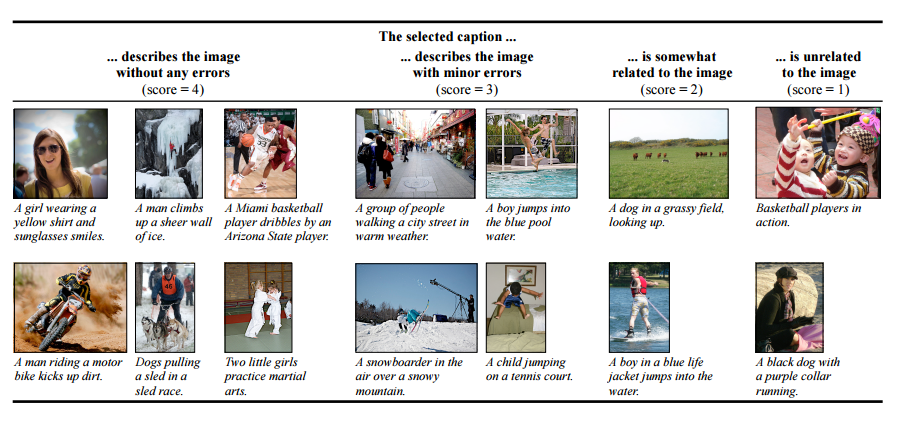
\includegraphics[scale=0.55]{Imgs/sentence_knn1.png}
\caption{نتایج کیفی اختصاص جملات و تصاویر به یک‌دیگر با استفاده از روش نزدیک‌ترین همسایه \cite{hodosh2013framing}}
\label{fig:knn1}
\end{figure}

به علاوه، جدول 
\ref{tbl:knn1}
نتایج ارزیابی روش نزدیک‌ترین همسایه را در اختصاص جملات و تصاویر به یک‌دیگر بر اساس سه معیار نمایش می‌دهد. معیار اول، میانگین امتیازی که افراد خبره به 1000 جملات تولید شده برای هر عکس داده‌اند را نمایش می‌دهد. این امتیازها اعداد صحیح بین ۱ تا ۴ را شامل می‌شوند و بیشینه ممکن برای این معیار، ۴ است. امتیاز بالاتر نشان‌دهنده مناسب‌تر بودن جملات تولید شده هستند. معیارهای \lr{BLUE} و \lr{ROUGE} معیارهایی هیتند که در پژوهش‌های ترجمه ماشین به عنوان محکی برای میزان خوب بودن ترجمه تولید شده، استفاده می‌شوند. مقادیر بالاتر در این معیارها، مناسب بودن عملکرد را نمایش می‌دهد. 

\begin{table}[h]
\center
\caption{نتایج استفاده از روش نزدیک‌ترین همسایه در اختصاص جملات و تصاویر \cite{hodosh2013framing}}
\label{tbl:knn1}
\begin{tabular}{c | c | c }
امتیاز افراد خبره & \lr{BLUE} & \lr{ROUGE}
\\
\hline
\hline
1.57 & 0.35 & 0.11\\
\end{tabular}
\end{table}

به عنوان یکی دیگر از روش‌های مورد استفاده در تولید خودکار شرح بر تصاویر، می‌توان به پژوهش ارائه شده در \cite{kuznetsova2012collective} اشاره کرد. در این پژوهش، تصاویر موجود در مجموعه‌داده، هر کدام با تعدادی عبارت زبانی که توسط کاربران انسانی نوشته شده‌اند، توصیف شده‌اند. در این پژوهش، هدف اصلی این است که با استخراج شبیه‌ترین عبارات موجود در مجموعه‌داده به تصویر ورودی و با کنارهم قرار دادن این عبارات و ساخت جمله با استفاده از چارچوب کاری مورد استفاده در پژوهش‌های تولید زبان طبیعی، جمله متناسب، تولید و نمایش داده‌شود.
\\
علاوه بر استفاده از روش نزدیک‌ترین همسایه برای انتخاب بهترین عبارات زبانی توصیف‌کننده تصویر، می‌توان از استفاده هوشمندانه از مرحله «برنامه‌ریزی محتوا»\enfootnote{Content Planning} در این پژوهش، به عنوان یکی از نقاط قوت آن، یاد کرد. این کار باعث می‌شود علاوه بر تولید جملات سازگار با یک‌دیگر، از تولید جملات تکراری در یک شرح بر یک تصویر، خودداری شود که از نقاط قوت این روش است. این مرحله با استفاده از روش‌های بهینه‌سازی انجام می‌شود. روش برنامه‌سازی خطی صحیح\enfootnote{Integer Linear Programming (ILP)}، به عنوان چارچوب کاری در این مرحله مورد استفاده قرار گرفته است.
\\
در این پژوهش، 89 کلاس از اجسام و 26 کلاس صحنه برای تشخیص محتوا انتخاب شده و تصاویر ورودی، با استفاده از آشکارکننده‌های فلزنسوالب، به این دسته‌ها اختصاص داده می‌شوند. این ‌کار، تخمین مناسبی از محتوای جملات ارائه می‌دهد. همین‌طور با استفاده از روش برچسب‌گذاری نقش کلمات در جمله\enfootnote{Part of Speech Tagging (POS Tagging)}، محتوای عبارات زبانی متناظر با جملات، به طریق مشابه، دسته‌بندی می‌شود.
\\
چهار دسته از عبارات برای هر تصویر ورودی، به این روش، استخراج می‌شود.

\begin{enumerate}
\item عبارات اسمی
\\
جستجوی عبارات اسمی موجود در مجموعه‌داده با استفاده از ویژگی بافت و رنگ به عنوان معیارهای محاسبه شباهت.
\\
مانند:
\begin{center}
\lr{
"The brown cow"
}
\end{center}
\item عبارات فعلی
\\
استفاده از معیارهای مشابه با عبارات اسمی در بین عبارات فعلی موجود در مجموعه‌داده
\\
مانند:
\begin{center}
\lr{
"boy running"
}
\end{center}
\item \enfootnote{Region/Stuff Prepositional Phrases}عبارات اضافی نواحی و اجسام
\\
جستجوی عبارات با استفاده از معیارهای شباهت رنگ، بافت، هیستوگرام گرادیان\enfootnote{Histogram of Gradient (HOG)} و همین‌طور با درنظر گرفتن ویژگی‌های هندسی اجسام
\\
مانند:
\begin{center}
\lr{
"in the sky" , "on the road"
}
\end{center}
\item عبارات اضافی صحنه\enfootnote{Scene Prepositional Pharases}
\\
جستجوی عبارات با استفاده از نتیجه دسته‌بندی صحنه با معیار $L^2$
\\
مانند:
\begin{center}
\lr{
"at the market" , "on hot summer day" , "in Sweden"
}
\end{center}
\end{enumerate}

 هر جمله شامل یک عبارت اسمی، بیان‌کننده مفعول جمله و یک یا چند نمونه از عبارتت دیگر بیان‌کننده مفهوم تصویر هستند. چهار نوع عملیات انتزاعی زیر برای ساخت جمله، در نظر گرفته شده است. هر یک از اعمال زیر با استفاده از روش برنامه‌سازی خطی صحیح، انجام می‌شوند.
 
\begin{enumerate}
 \item انتخاب مجموعه مفعولی که نیاز به توصیف دارند (هر مفعول برای یک جمله)
 \item بازچینی و ترتیب‌دهی به مفعول‌ها
 \item انتخاب مجموعه‌ عبارات مورد نیاز برای هر جمله
 \item بازچینی و ترتیب‌دهی عبارات در هر جمله
\end{enumerate}

در شکل \ref{fig:knn2}، نتایج عملکرد الگوریتم را در مقایسه با جملات تولید شده توسط انسان، مشاهده می‌نمایید. مواردی که با عبارت \lr{ILP} مشخص شده‌اند، خروجی‌های روش برنامه‌سازی خطی صحیح و مواردی که با عبارت \lr{HMM} نمایش داده شده‌اند، جملات تولید شده توسط انسان را نمایش می‌دهند.

\begin{figure}[H]
\center
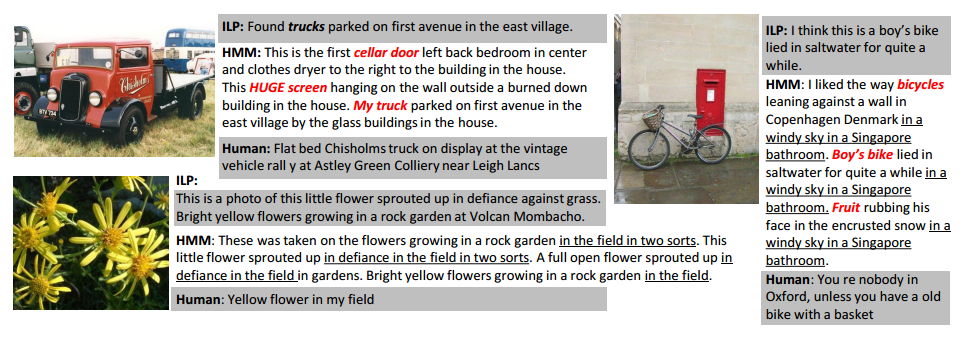
\includegraphics[scale=0.5]{Imgs/sentence_knn2.png}
\caption{نتایج برنامه‌سازی خطی صحیح در مقایسه با جملات تولید شده انسان \cite{kuznetsova2012collective}}
\label{fig:knn2}
\end{figure}

به علاوه، در شکل \ref{fig:knn3}، مواردی را مشاهده می‌نمایید که در آن‌ها، خروجی الگورتیم نسبت به جملات تولید شده توسط انسان، برتری دارد.


\begin{figure}[H]
\center
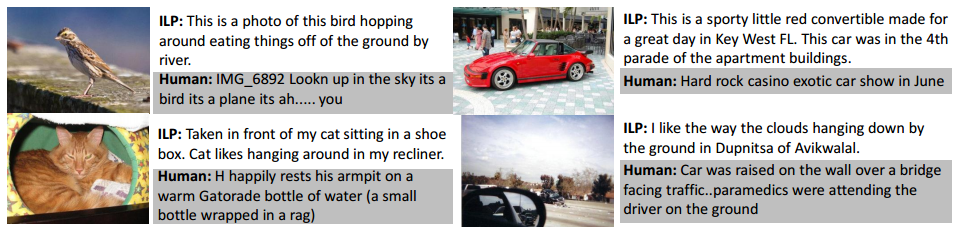
\includegraphics[scale=0.5]{Imgs/sentence_knn3.png}
\caption{مواردی از خروجی برنامه‌سازی خطی صحیح که نسبت به جملات انسان، برتری دارد \cite{kuznetsova2012collective}.}
\label{fig:knn3}
\end{figure}

با وجود این‌که الگوریتم در برخی موارد کارایی بهتری از خود نشان داده‌ است، جملاتی نیز وجود دارند که به لحاظ دستور زبان، عدم شناخت صحیح یا ناسازگاری محتوایی دچار مشکل شده‌اند. شکل \ref{fig:knn4}، نمونه‌هایی از این دست را نمایش می‌دهد.


\begin{figure}[H]
\center
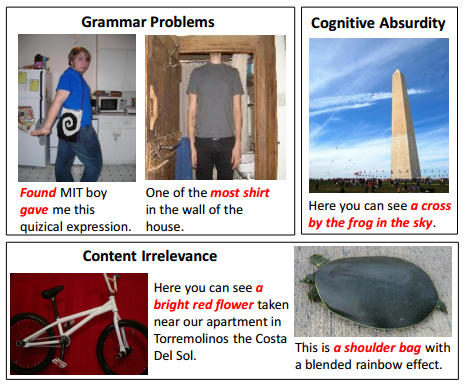
\includegraphics[scale=0.6]{Imgs/sentence_knn4.png}
\caption{نتایج برنامه‌سازی خطی صحیح که به لحاظ‌های مختلف دچار مشکل شده‌اند \cite{kuznetsova2012collective}.}
\label{fig:knn4}
\end{figure}

%%%%%%%%%%%%%%%%%%%%%%%%%%%%%%%%%%%%%%%%%%%%%%%%%%%%%%%%%%
\subsection{استفاده از قالب‌های آماده زبانی}

یکی دیگر از روش‌هایی که برای تولید جمله متناظر با یک تصویر مورد استفاده قرار می‌گیرد، روش استفاده از قالب‌های آماده زبانی است. پژوهش‌هایی که از این روش برای تولید جملات زبانی استفاده کرده‌اند، غالبا پژوهش‌های وظیفه‌‌محور\enfootnote{Task-Based} هستند. حملات تولید شده در این پژوهش‌ها عموما به طور هدف‌مند برای پاسخ دادن به موارد معینی تولید می‌شوند و قابلیت تعمیم‌پذیری کم‌تری نسبت به روش‌های دیگر دارند.
\\
به عنوان مثال در پژوهش \cite{gupta2012image}، یک روش مبتنی بر استفاده از قالب‌های آماده زبانی برای تولید خودکار شرح بر تصاویر ارائه شده است. جملاتی که در این پژوهش تولید می‌شوند، باید قادر به مشخص کردن اطلاعات زیر برای هر تصویر باشند:
\begin{enumerate}
\item اجسامی که در تصویر مشاهده می‌شوند
\item ويژگی‌های اجسام شامل رنگ، اندازه و موارد مشابه
\item فاعل
\item فعل
\item حروف اضافه
\end{enumerate}

در این پژوهش، هدف اصلی این است که پس از برجسب‌زدن تصویر با استفاده از روش‌‌های موجود در حاشیه‌نویسی تصویر\enfootnote{Image Annotation}، که در آن‌ها هر تصویر با یک یا چند برچسب زبانی حاشیه نویسی می‌شود، بتوان جمله‌های بیان‌کننده موارد فوق را در تصویر با استفاده از برچسب‌های تولید شده، تولید نمود.
در این پژوهش از مجموعه‌داده \lr{PASCAL}\enfootnote{\url{http://vision.cs.uiuc.edu/pascal-sentences/}{http://vision.cs.uiuc.edu/pascal-sentences/}} استفاده شده است که شامل 1000 تصویر و برای هر تصویر، ۵ جمله تولید شده توسط انسان است. 
\\
ابتدا با استفاده از یک ابزار برچسب‌زنی نقش کلمات در جملات، تمام کلمات موجود در جملات مجموعه‌داده، برچسب‌ زده می‌شوند. سپس برای هر تصویر، ۲ مفعول از بین ۵ جمله متناظر آن و برای هر مفعول، یک ویژگی استخراج می‌شود. به علاوه با استفاده از نرم‌افزار \lr{WordNet}، مترادف‌های هر یک از کلمات استخراج شده، تا ۳ سطح، یافت می‌شوند.
\\
در مرحله بعدی برای یافتن فاعل جمله، کافیست تعداد دفعاتی را که هر یک از ۲ مفعول استخراج شده، در بین 5 جمله موجود، در نقش فاعل بوده‌اند شمرده و کلمه‌ای را که بیشترین تعداد تکرار به عنوان فاعل را داشته است، به عنوان فاعل جمله در نظر بگیریم. با مشخص شدن فاعل و مفعول جمله، کافیست فعل مورد نظر را با شمارش تعداد دفعات تکرار افعال مختلف در جملاتی که فاعل و مفعولشان برابر با مورد در حال بررسی است، فعل با بیشترین تکرار را انتخاب کنیم. اگر چنین فعلی یافت نشد، از فعل در قالب آماده استفاده نخواهد شد.
\\
موارد مورد نیاز دیگر نیز به همین ترتیب استخراج می‌شوند. در انتها، با توجه به پیدا شدن یا نشدن فعل و همین‌طور نوع فعل استخراج شده، از یکی از قالب‌های زیر برای ساخت جمله استفاده می‌شود.
\begin{enumerate}
\item فعل اصلی استخراج شده است:
\begin{center}
(معرف ۱ - ویژگی ۱ - فاعل) - فعل - حرف اضافه - (معرف ۲ - ویژگی ۲ - مفعول)
\end{center}
\item فعل گذرا استخراج شده است:
\begin{center}
(معرف ۱ - ویژگی ۱ - فاعل) - فعل - (معرف ۲ - ویژگی ۲ - مفعول)
\end{center}
\item فعلی یافت نشده است:
\begin{center}
(معرف ۱ - ویژگی ۱ - فاعل) - حرف اضافه - (معرف ۲ - ویژگی ۲ - مفعول)
\end{center}
\end{enumerate}

شکل \ref{fig:temp1} مواردی از جملات تولید شده برای تصاویر موجود در مجموعه‌داده را نمایش می‌دهد. نمونه‌هایی که در این شکل مشاهده می‌شود، نمونه‌هایی هستند که به لحاظ معنایی صحیح بوده و با تصویر مربوطه سازگاری دارند.

\begin{figure}[H]
\center
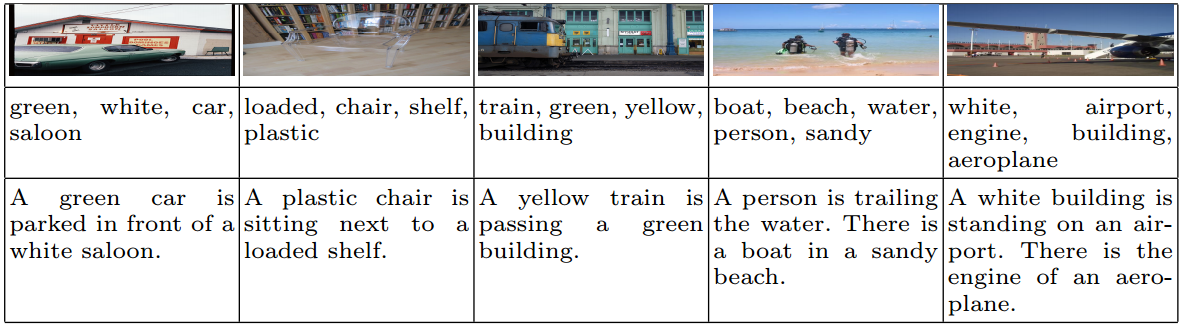
\includegraphics[scale=0.4]{Imgs/sentence_template1.png}
\caption{نمونه‌های صحیح از جملات تولید شده توسط قالب‌های آماده زبانی\cite{gupta2012image}}
\label{fig:temp1}
\end{figure}

به علاوه در شکل \ref{fig:temp2}، نمونه‌هایی از خروجی الگوریتم را در حالاتی که جملات تولید شده به لحاظ شناخت صحیح فاعل، ویژگی، فعل، حروف اضافه و همین‌طور تکرار کلمات در جمله دچار مشکل شده‌اند، نمایش می‌دهد.

\begin{figure}[H]
\center
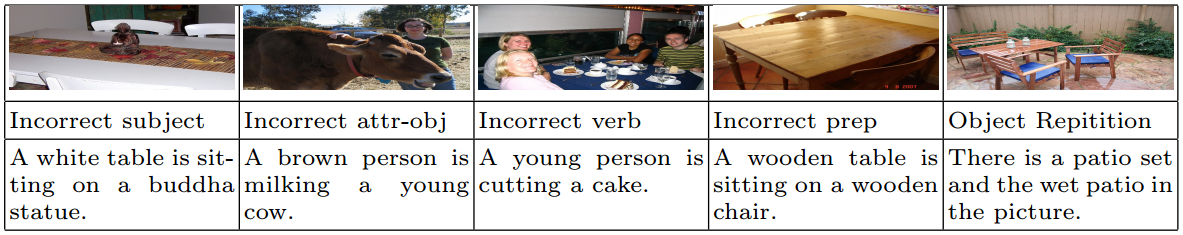
\includegraphics[scale=0.4]{Imgs/sentence_template2.png}
\caption{نمونه‌های اشتباه تولید شده توسط قالب‌های آماده زبانی\cite{gupta2012image}}
\label{fig:temp2}
\end{figure}

علاوه بر این، جدول \ref{tbl:temp1}، نتایج معیار \lr{BLUE} را در حالات مختلف (استفاده از ترکیبات چندتایی کلمات\enfootnote{n-grams}) نمایش می‌دهد. همان‌طور که مشاهده می‌شود، مقادیر به‌دست آمده از این معیارها، قابل قبول بودن دقت جملات تولید شده توسط این روش را نمایش می‌دهند. در ستون‌هایی از جدول که از حرف \lr{s} استفاده شده، تطابق بین کلمات هم‌معنی نیز در نظر گرفته شده است در صورتی‌که در بقیه ستون‌ها، کلمات دقیق با هم مقایسه شده‌اند. همان‌طور که مشخص است، استفاده از کلمات هم‌معنی نتایج بهتری را ارائه داده است.

\begin{table}[H]
\center
\caption{نتایج معیارهای \lr{BLUE} و \lr{ROUGE} درحالات مختلف \cite{gupta2012image}}
\label{tbl:temp1}
\begin{tabular}{c | c | c | c | c | c | c | c}
\lr{BLUE-1} & \lr{BLUE-1-s} & \lr{BLUE-2} & \lr{BLUE-2-s} & \lr{BLUE-3} & \lr{BLUE-3-s} & \lr{ROUGE-1} & \lr{ROUGE-1-s} 
\\
\hline
\hline
0.74 & 0.79 & 0.55 & 0.61 & 0.35 & 0.42 & 0.55 & 0.60 \\
\end{tabular}
\end{table}

%%%%%%%%%%%%%%%%%%%%%%%%%%%%%%%%%%%%%%%%%%%%%%%%%%%%%%%%%%%
%\subsection{روش‌های مبتنی بر مدل‌های آماری}
%
%%%%%%%%%%%%%%%%%%%%%%%%%%%%%%%%%%%%%%%%%%%%%%%%%%%%%%%%%%%
%\subsection{روش‌های صوری}
%
%%%%%%%%%%%%%%%%%%%%%%%%%%%%%%%%%%%%%%%%%%%%%%%%%%%%%%%%%%
\subsection{روش‌های مبتنی بر شبکه‌های عصبی بازگشتی}

%%%%%%%%%%%%%%%%%%%%%%%%%%%%%%%%%%%%%%%%%%%%%%%%%%%%%%%%%%
\subsection{جمع‌بندی}
